
\newpage
\section{Use case diagrams e casi d'uso}

\begin{figure}[h!]
    \centerline{\includesvg[width=1\linewidth]{img/UseCase/UseCase-Diagram.svg}}
    \caption{Use Case diagram}
    \label{fig:useCase}
\end{figure}

\newpage
\subsection{Use case table $-$ Utente non autenticato e Cliente}

\begin{figure}[h!]
    \centering
    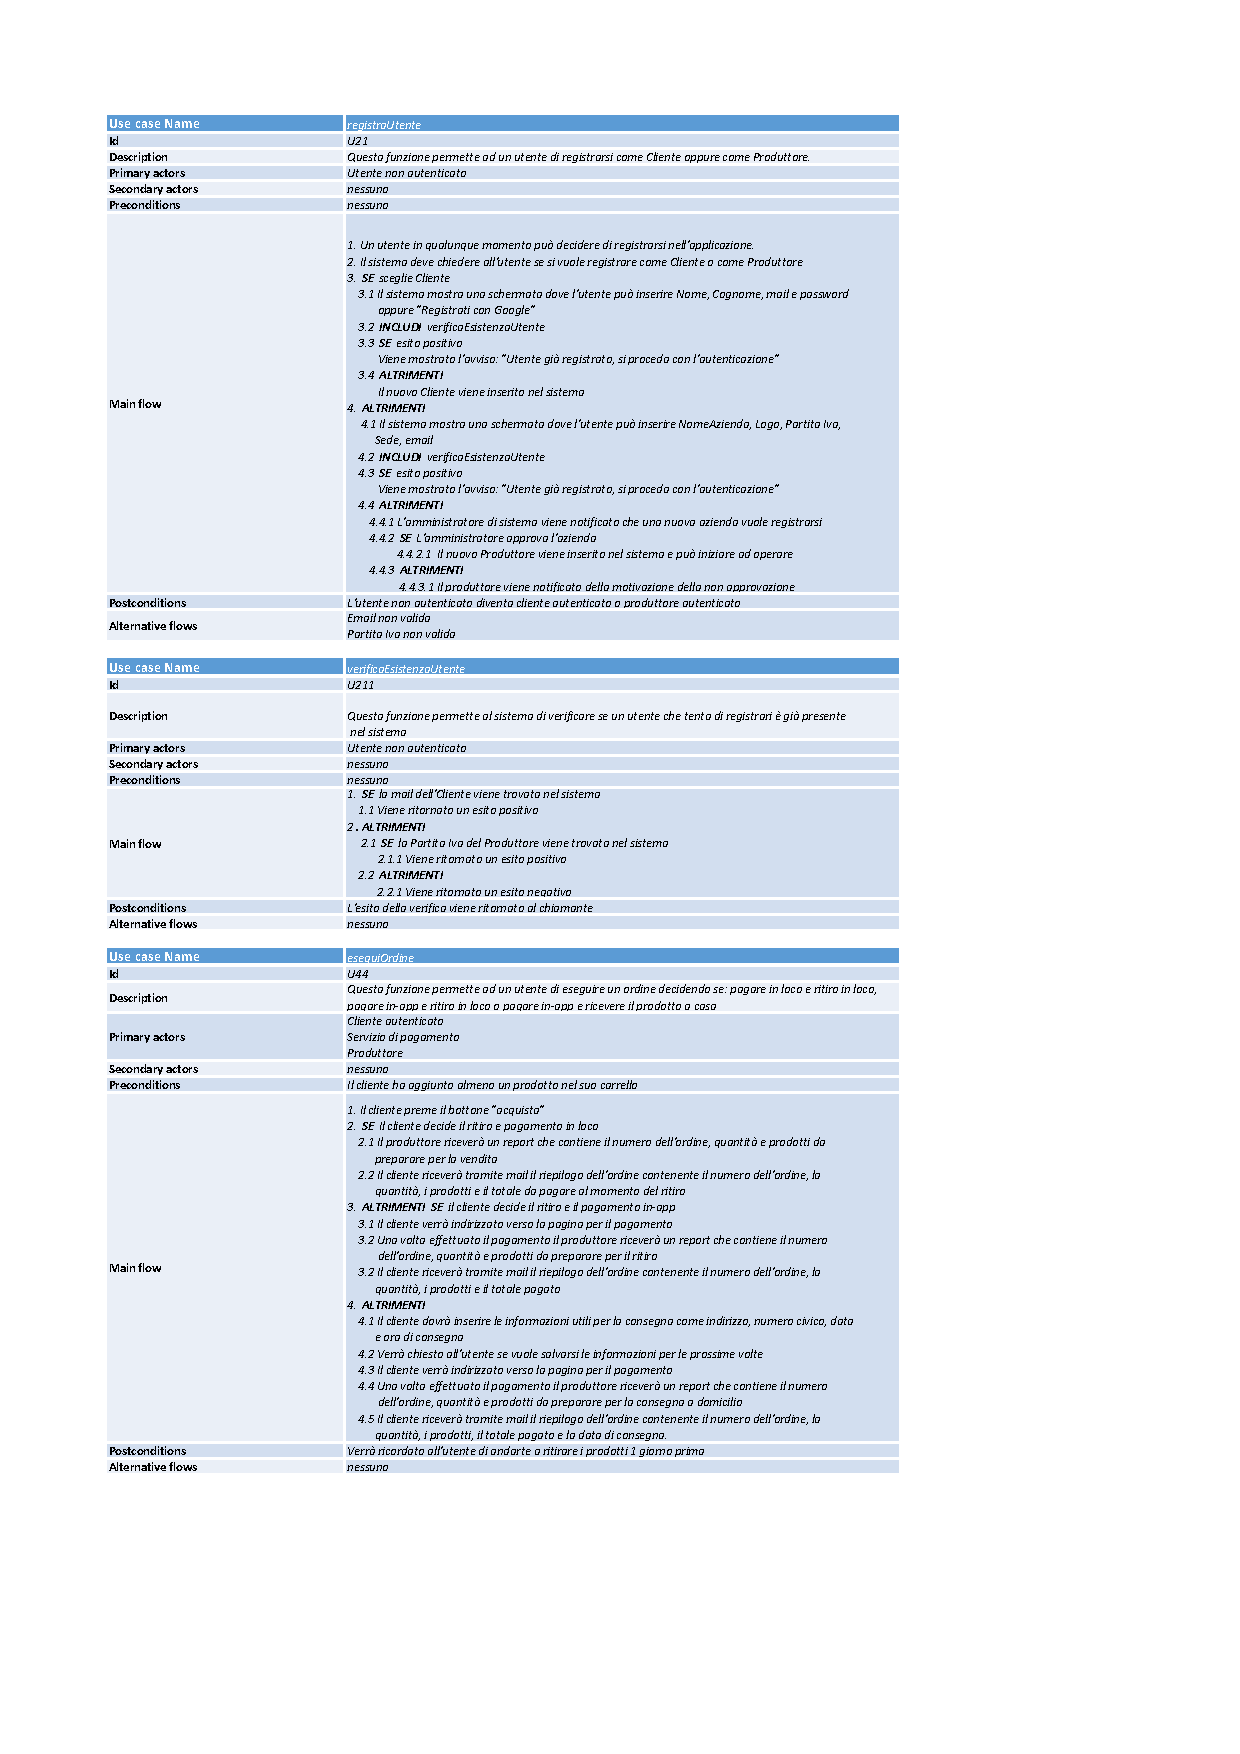
\includegraphics[trim= 1.8cm 4.3cm 5cm 1.9cm, clip]{Deliverables/first-deliverable/img/UseCase/UseCase-Table-Client.pdf}
\end{figure}

\newpage
\subsection{Use case table $-$ Produttore}
\begin{figure}[h!]
    \centering
    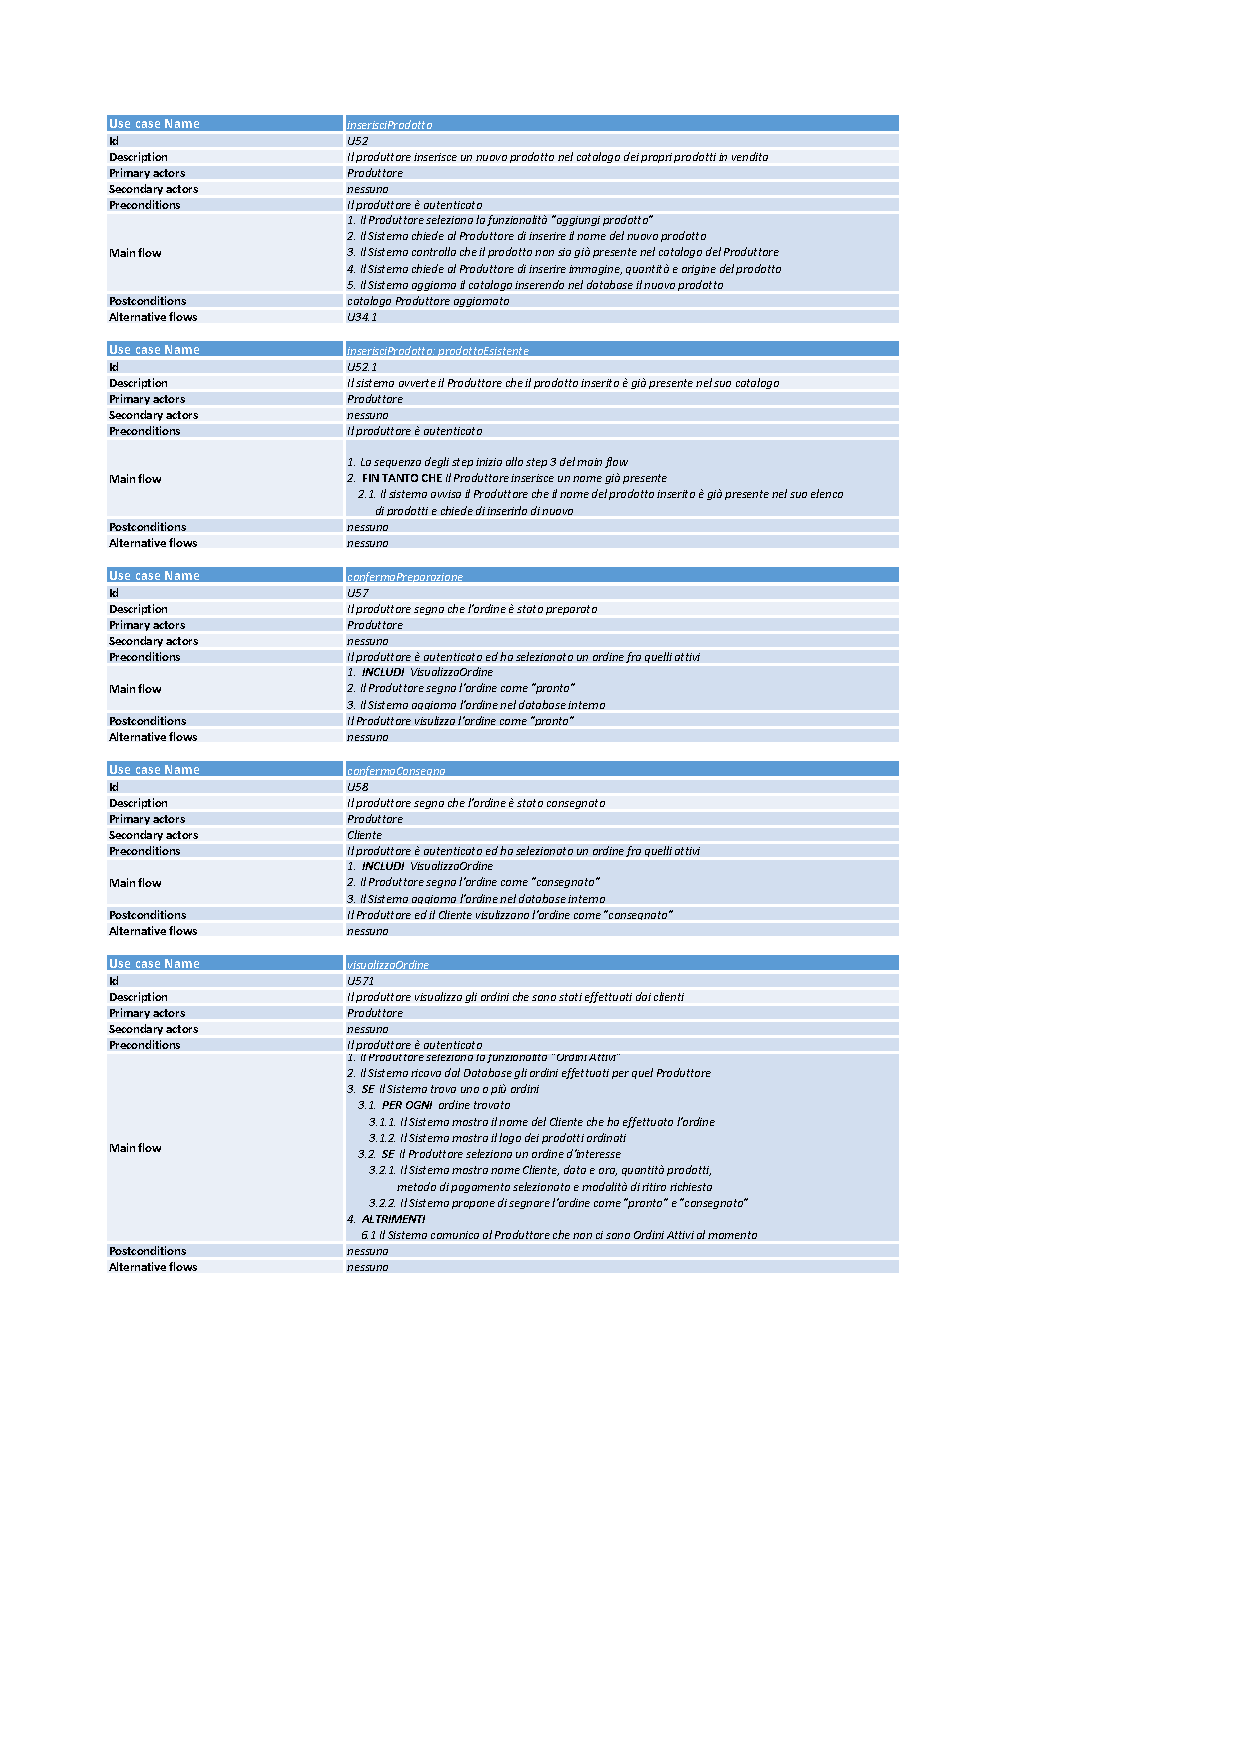
\includegraphics[trim= 1.8cm 8cm 5cm 1.9cm, clip]{Deliverables/first-deliverable/img/UseCase/UseCase-Table-Producer.pdf}
\end{figure}

\newpage
\subsection{Use case table $-$ Amministratore}
\begin{figure}[h!]
    \centering
    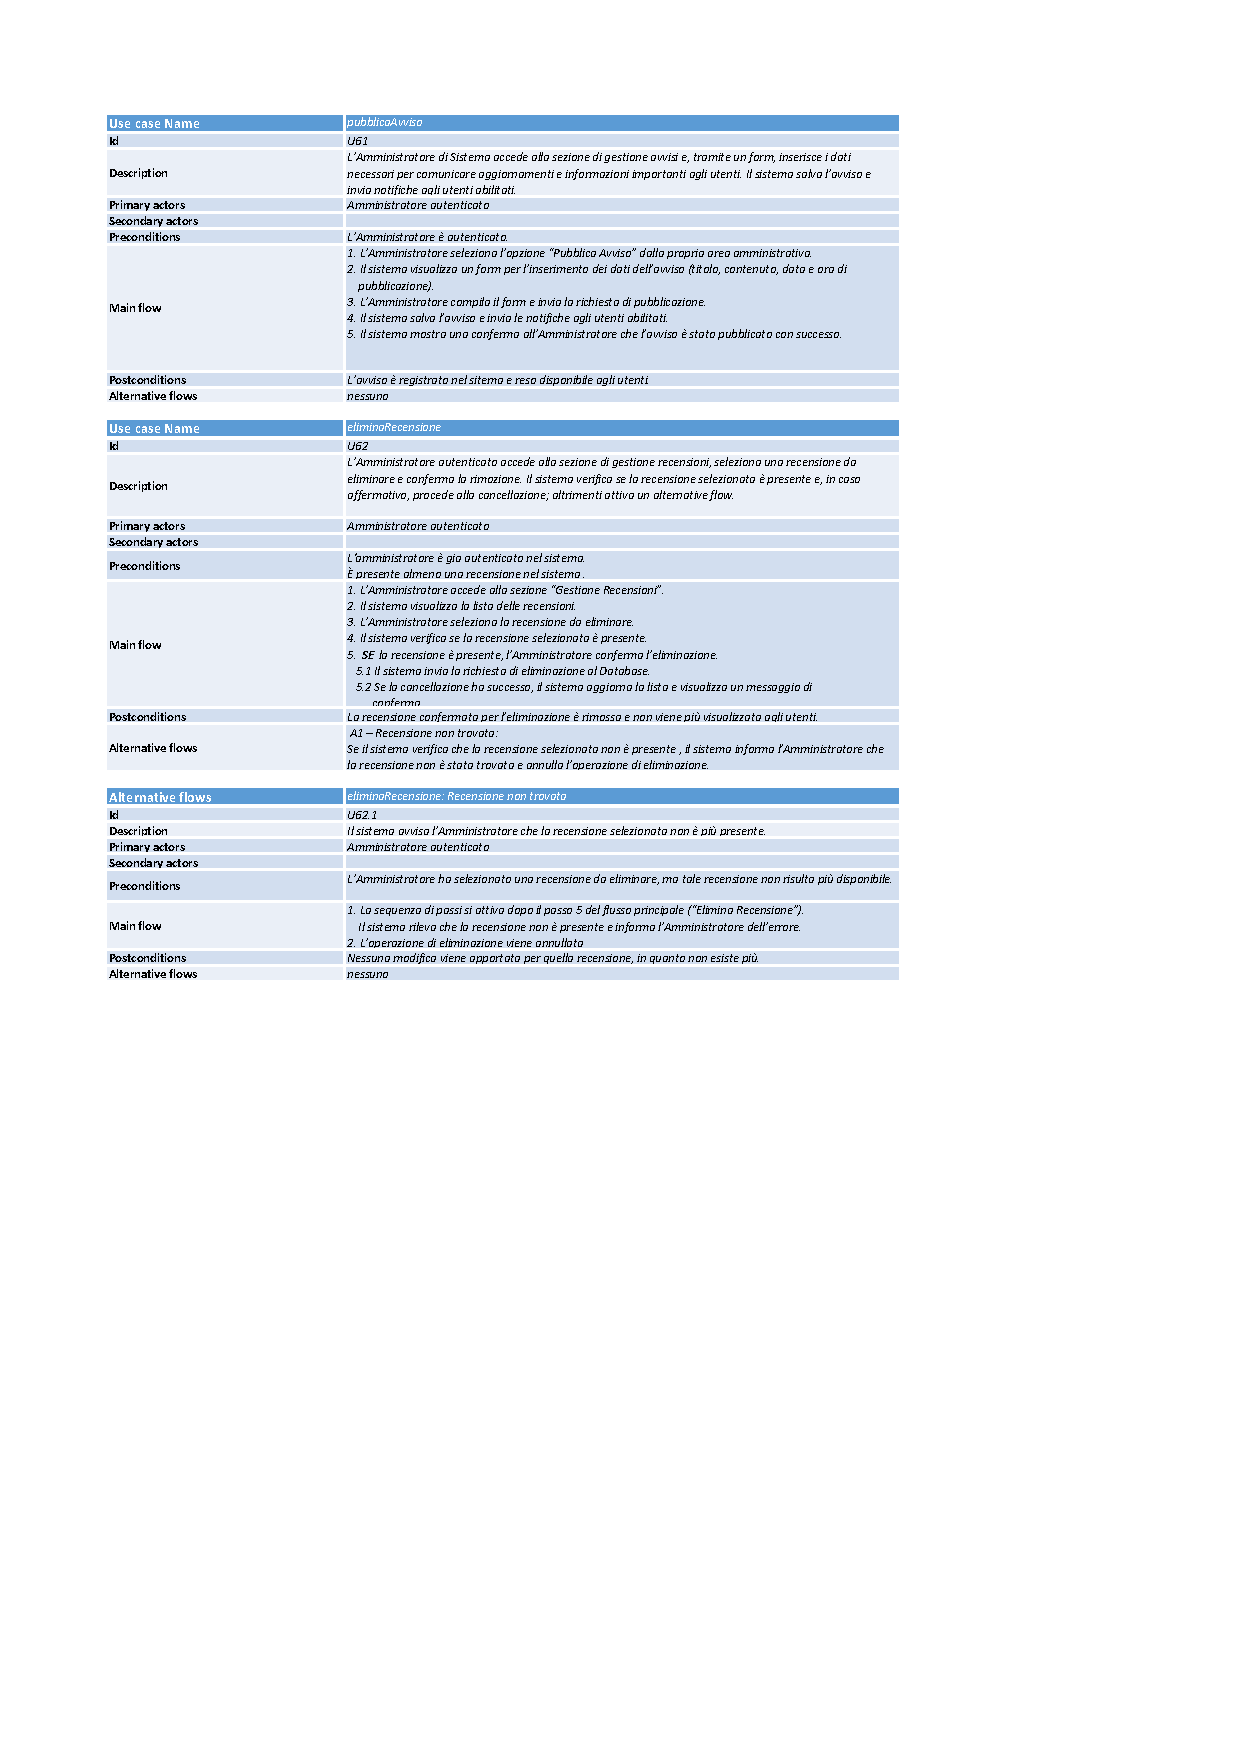
\includegraphics[trim= 1.8cm 13cm 5cm 1.9cm, clip]{Deliverables/first-deliverable/img/UseCase/UseCase-Table-Amministrator.pdf}
\end{figure}

\paragraph{Numerazione degli Use Case}

Gli \textbf{id} utilizzati nelle tabelle mostrate sopra sono stati così calcolati.

Prendiamo come esempio \textit{cercaProdotti}, \textit{modificaDatiAccount}, \textit{visualizzaProdotto} e \textit{visualizzaSegnalazioni} che si trovano nello Use Case diagram nella Figura \ref{fig:useCase}:



\begin{itemize}
    \item \textbf{cercaProdotti}: avrà come id 11 essendo che è il primo attore e che cercaProdotti è il primo use case per quell'attore.
    \item \textbf{modificaDatiAccount}: avrà come id 31 essendo che è il terzo attore e che modificaDatiAccount è il primo, e unico, use case per quell'attore
    \item \textbf{visualizzaProdotto}: avrà come id 551 essendo che è il quinto attore, il quinto use case di quell'attore e che è il primo use case associato a \textit{modificaProdotto}
    \item \textbf{visualizzaSegnalazioni}: avrà come id 63, stesso ragionamento per i precedenti, sesto attore e terzo use case associato all'attore.
\end{itemize}





